\documentclass[tikz,border=0pt]{standalone}
\usepackage{amsmath}
\usetikzlibrary{backgrounds}
\definecolor{latar}{HTML}{171D2B}
\definecolor{aksen}{HTML}{F7B538}
\definecolor{teks}{HTML}{FFFFFF}
\definecolor{garis}{HTML}{2A3448}
\begin{document}
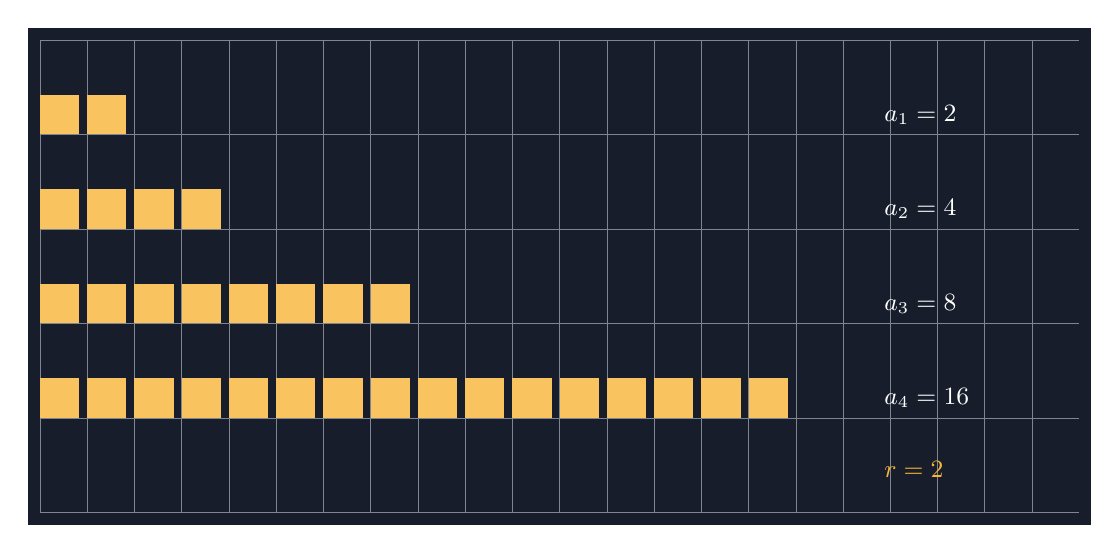
\begin{tikzpicture}[background rectangle/.style={fill=latar}, show background rectangle]
% grid halus
\foreach \x in {0,0.6,...,13.2} \draw[garis!60,very thin] (\x,0.4) -- (\x,-5.6);
\foreach \y in {0.4,-0.8,...,-5.6} \draw[garis!60,very thin] (0,\y) -- (13.2,\y);
% baris barisan geometri a1=2, r=2
\foreach \n/\jmlh in {1/2, 2/4, 3/8, 4/16} {
  \foreach \k in {1,...,\jmlh}
    \fill[aksen!80] ({(\k-1)*0.6}, {-\n*1.2+0.4}) rectangle ++(0.5,0.5);
  \node[teks,font=\small,anchor=west] at (10.6, {-\n*1.2+0.65}) {$a_{\n} = \jmlh$};
}
% label rasio
\node[aksen,font=\small,anchor=west] at (10.6,-5.05) {$r=2$};
\end{tikzpicture}
\end{document}
